\documentclass[xcolor=svgnames]{beamer}
\usecolortheme[named=blue]{structure}
\usetheme{theme1}
\usepackage{amsmath}
\usepackage{amssymb}
\usepackage{verbatim}
\usepackage{graphicx}
\usepackage{xcolor}
\usepackage{hyperref}
\usepackage{showexpl}
\lstloadlanguages{[LaTeX]Tex}
\lstset{
    explpreset={numbers=none,pos=b},
    basicstyle=\ttfamily\small,
    commentstyle=\itshape\ttfamily\small,
    breaklines=false,
    preset=\let\label\orilabel,
    columns=flexible
}
\usepackage{array}
\usepackage[backend=bibtex,bibstyle=numeric-comp]{biblatex}
\newcommand{\putCitation}[2]{\footnotetext[#1]{\tiny{\citeauthor{#2} \citefield{#2}{shortjournal} \textbf{\citefield{#2}{volume}}, \citefield{#2}{pages} (\citeyear{#2})}}}
\newcommand{\putCitations}[3]{\footnotetext[#1]{\tiny{\citeauthor{#2} \citefield{#2}{shortjournal} \textbf{\citefield{#2}{volume}}, \citefield{#2}{pages} (\citeyear{#2}); \citeauthor{#3} \citefield{#3}{shortjournal} \textbf{\citefield{#3}{volume}}, \citefield{#3}{pages} (\citeyear{#3})}}}

\title{AWK From My Perspective}
\author{Ramachandran Subramanian}
\institute[UB]{
    Computational Sciences Club
}
\date{September 21, 2016}

\begin{document}
\let\orilabel\label
%\maketitle
{
    \setbeamertemplate{footline}{}
    \begin{frame}
        \titlepage
    \end{frame}
}
\addtocounter{framenumber}{-1}

\section{Contents}
\begin{frame}
    \frametitle{Assumptions and disclaimer}
    \begin{itemize}
        \visible<1->{\item Assumptions: Familiarity with Linux/Unix/Bash commands and basic programming knowledge.}
        \visible<2->{\item Disclaimer: This is strictly AWK from my perspective. I might not cover all different aspects of it in detail (gawk, regular expressions, arrays, debugging, output formatting, built-in and user-defined functions etc.) and what I do cover might not be the most efficient way to do a certain task. This workshop is therefore intended as an introductory workshop to give you a flavor of the convenience and versatility of AWK.}
        \visible<3->{\item Reference and further reading: https://www.gnu.org/software/gawk/manual/gawk.html}
    \end{itemize}
\end{frame}
\begin{frame}
    \frametitle{Overview of the workshop}
    \begin{itemize}
        \item Basics of using AWK - syntax, BEGIN/END blocks and predefined variables
        \item AWK in the command line. Input from files and pipes. Few use and throw examples that demonstrate the power of AWK.
        \item Writing AWK scripts in a separate file.
    \end{itemize}
\end{frame}
\section{Introduction}
\begin{frame}
    \frametitle{AWK basics}
    \begin{itemize}
        \item Syntax: awk `/pattern/ {command}' input-stream.
        \item Reads the entire input stream (file(s) or pipe) and looks for the given pattern and executes the command on that record.
        \item Usually every line is considered a record and every column is considered a field.
        \item Default: record separator is the newline character and the field separator is white-space sequences (spaces, tabs and newlines).
        \item Field values are referenced using the dollar symbol `\$'. \$0 represents the entire record. `print \$0' (is the same as `print') is the default if no command is specified.
    \end{itemize}
\end{frame}
\begin{frame}
    \frametitle{Some predefined variables - command line examples}
    \begin{itemize}
        \item NR - total number of records processed until this point. Gets updated each time AWK reads a record.
        \item NF - total number of fields in the current record. Value of NF gets reset to 0 before processing the next record.
        \item FS - field separator (default: white-space sequences).
        \item RS - record separator (default: newline character).
    \end{itemize}
\end{frame}
\begin{frame}
    \frametitle{Key aspects - command line examples}
    \begin{columns}
        \begin{column}[T]{7cm}
            \begin{itemize}
                \item BEGIN block - gets executed only once before the first record is read. All predefined variables are either 0, not defined or null depending on context.
                \item END block - gets executed only once after processing all the input.
                \item The `next' statement - stops reading current record and proceeds to the next record.
                \item Assigning a value to a variable.
            \end{itemize}
        \end{column}
        \begin{column}[T]{4cm}
            \begin{figure}
                \begin{center}
                    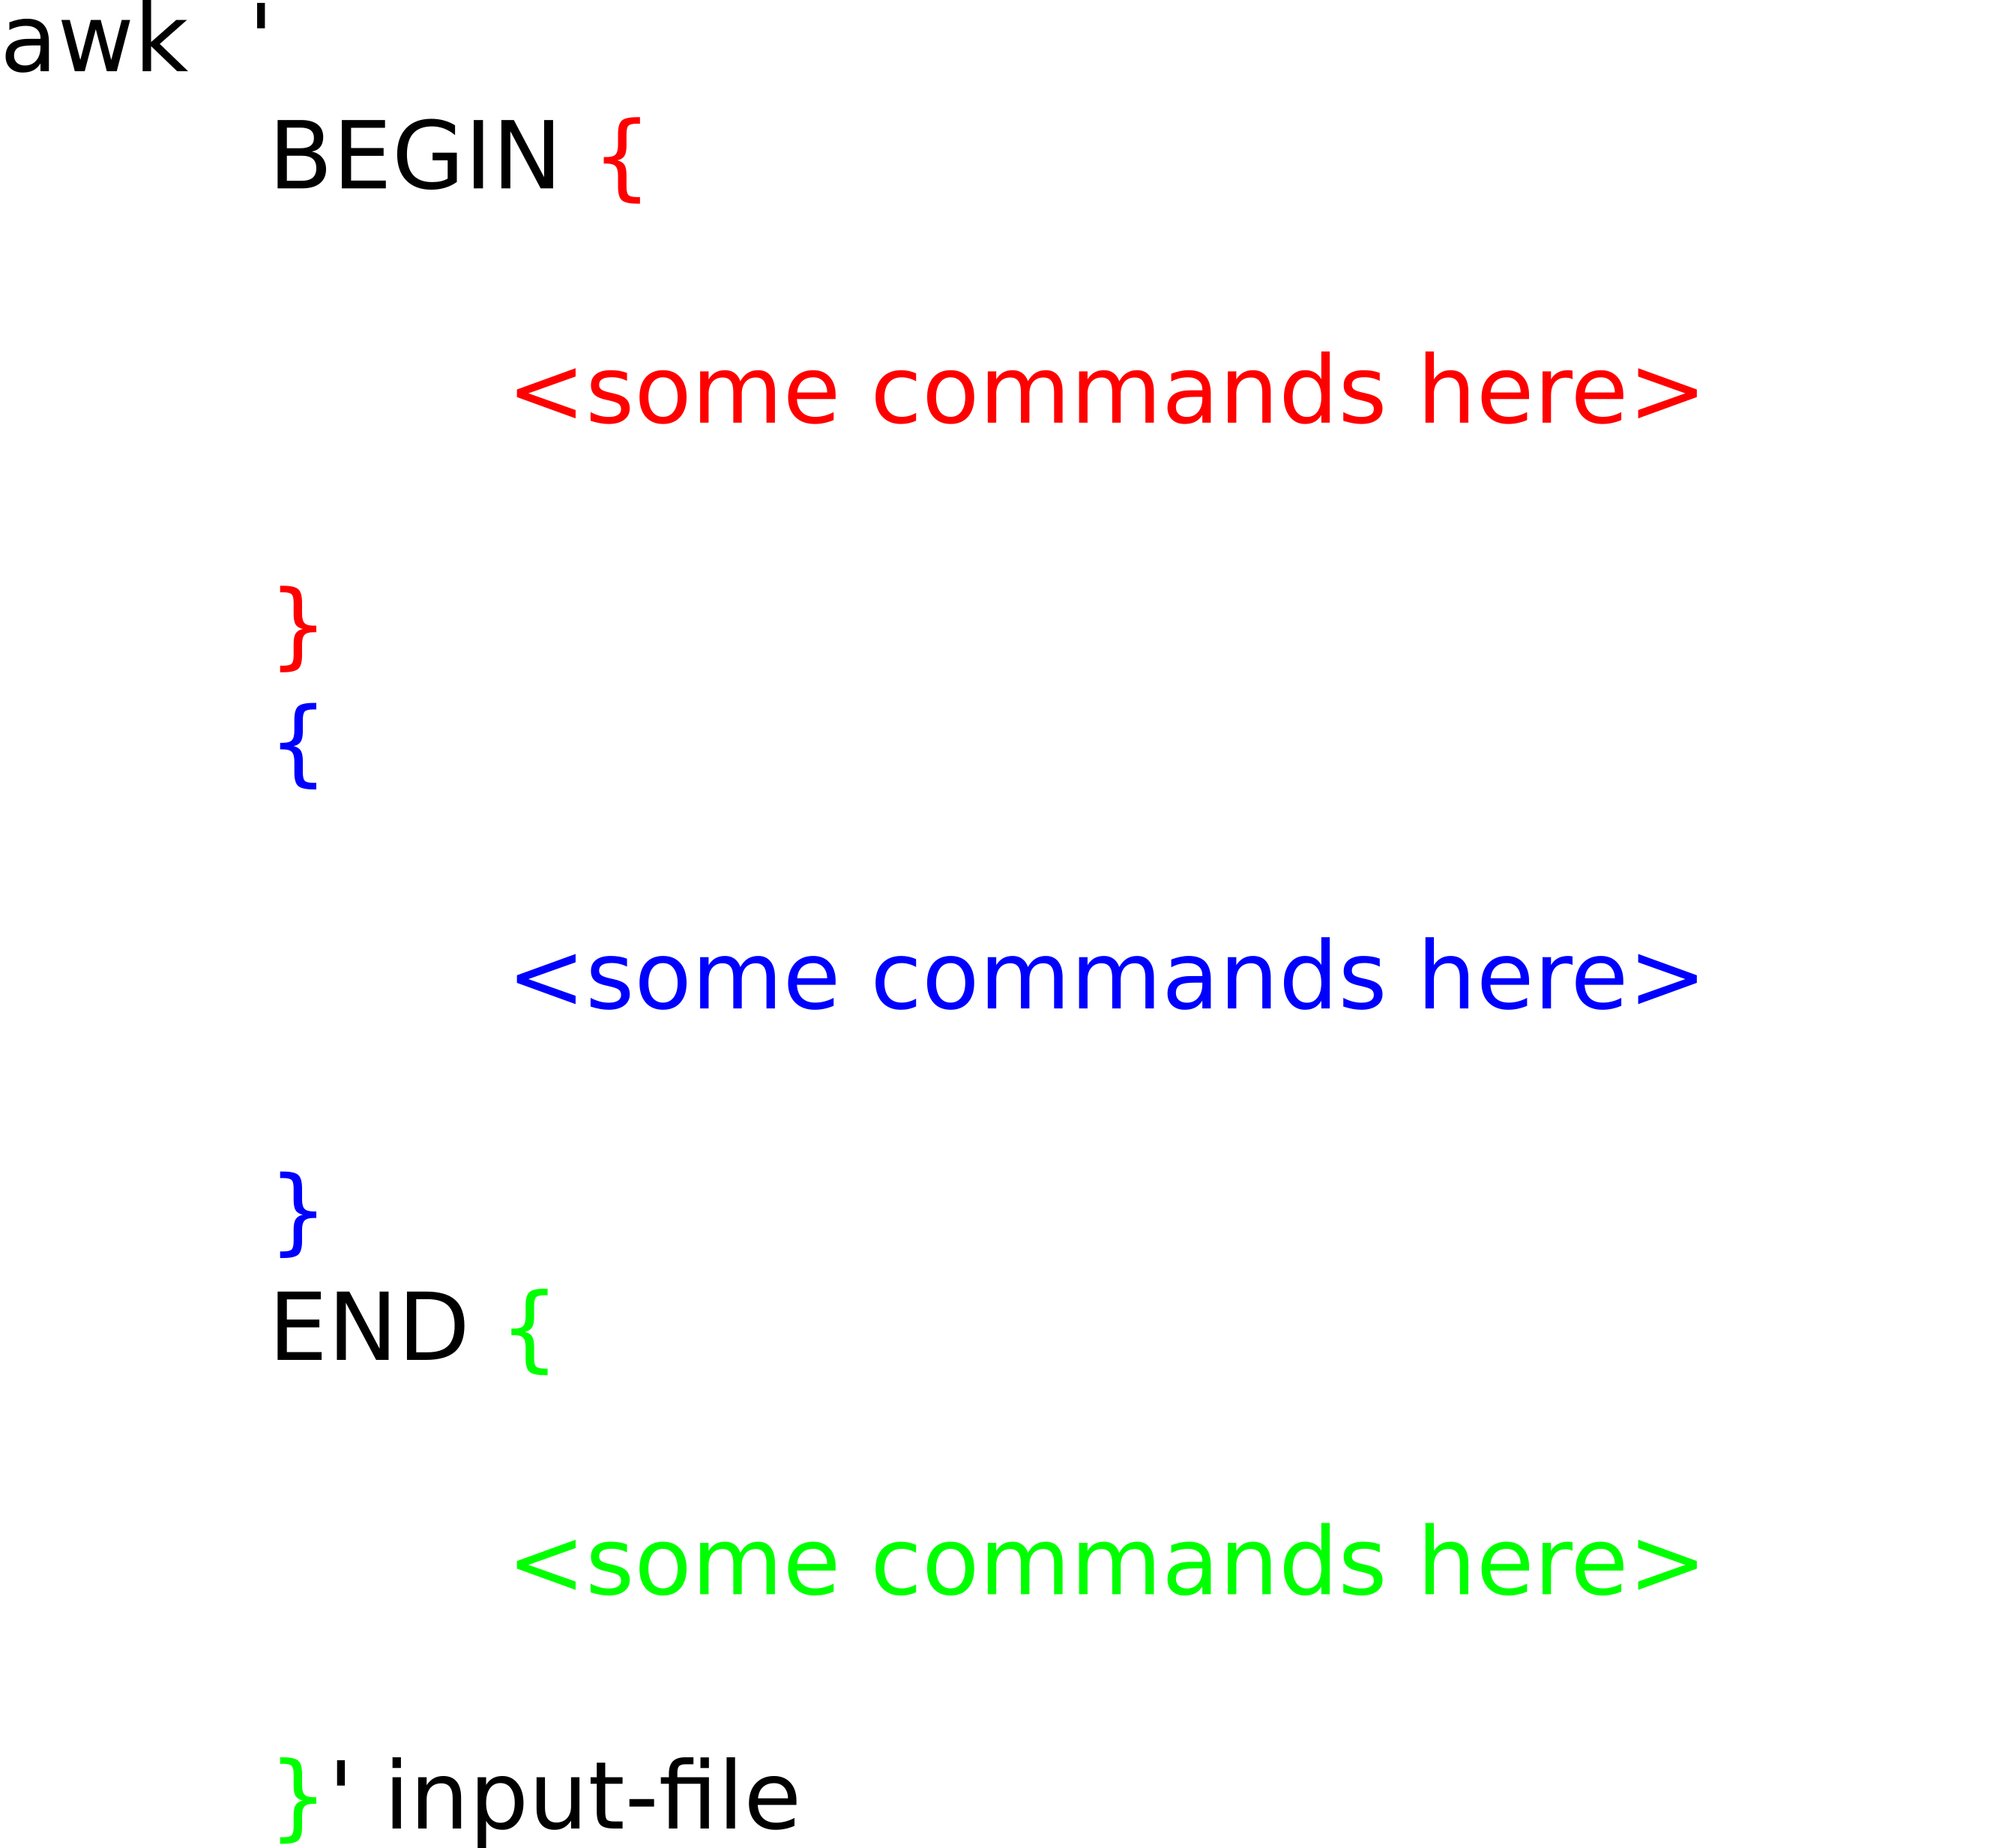
\includegraphics[scale=0.22,keepaspectratio]{awkSingleInput.png}
                \end{center}
            \end{figure}
        \end{column}
    \end{columns}

\end{frame}

\begin{frame}
    \frametitle{Pipe as input instead of a file - command line examples}
    \begin{itemize}
        \item Using BEGIN block as a calculator.
        \item Total size of files in a directory.
        \item Canceling specific jobs in CCR.
    \end{itemize}
\end{frame}

\begin{frame}
    \frametitle{Multiple input files}
    Order of execution of statements:
    \begin{figure}
        \centering
        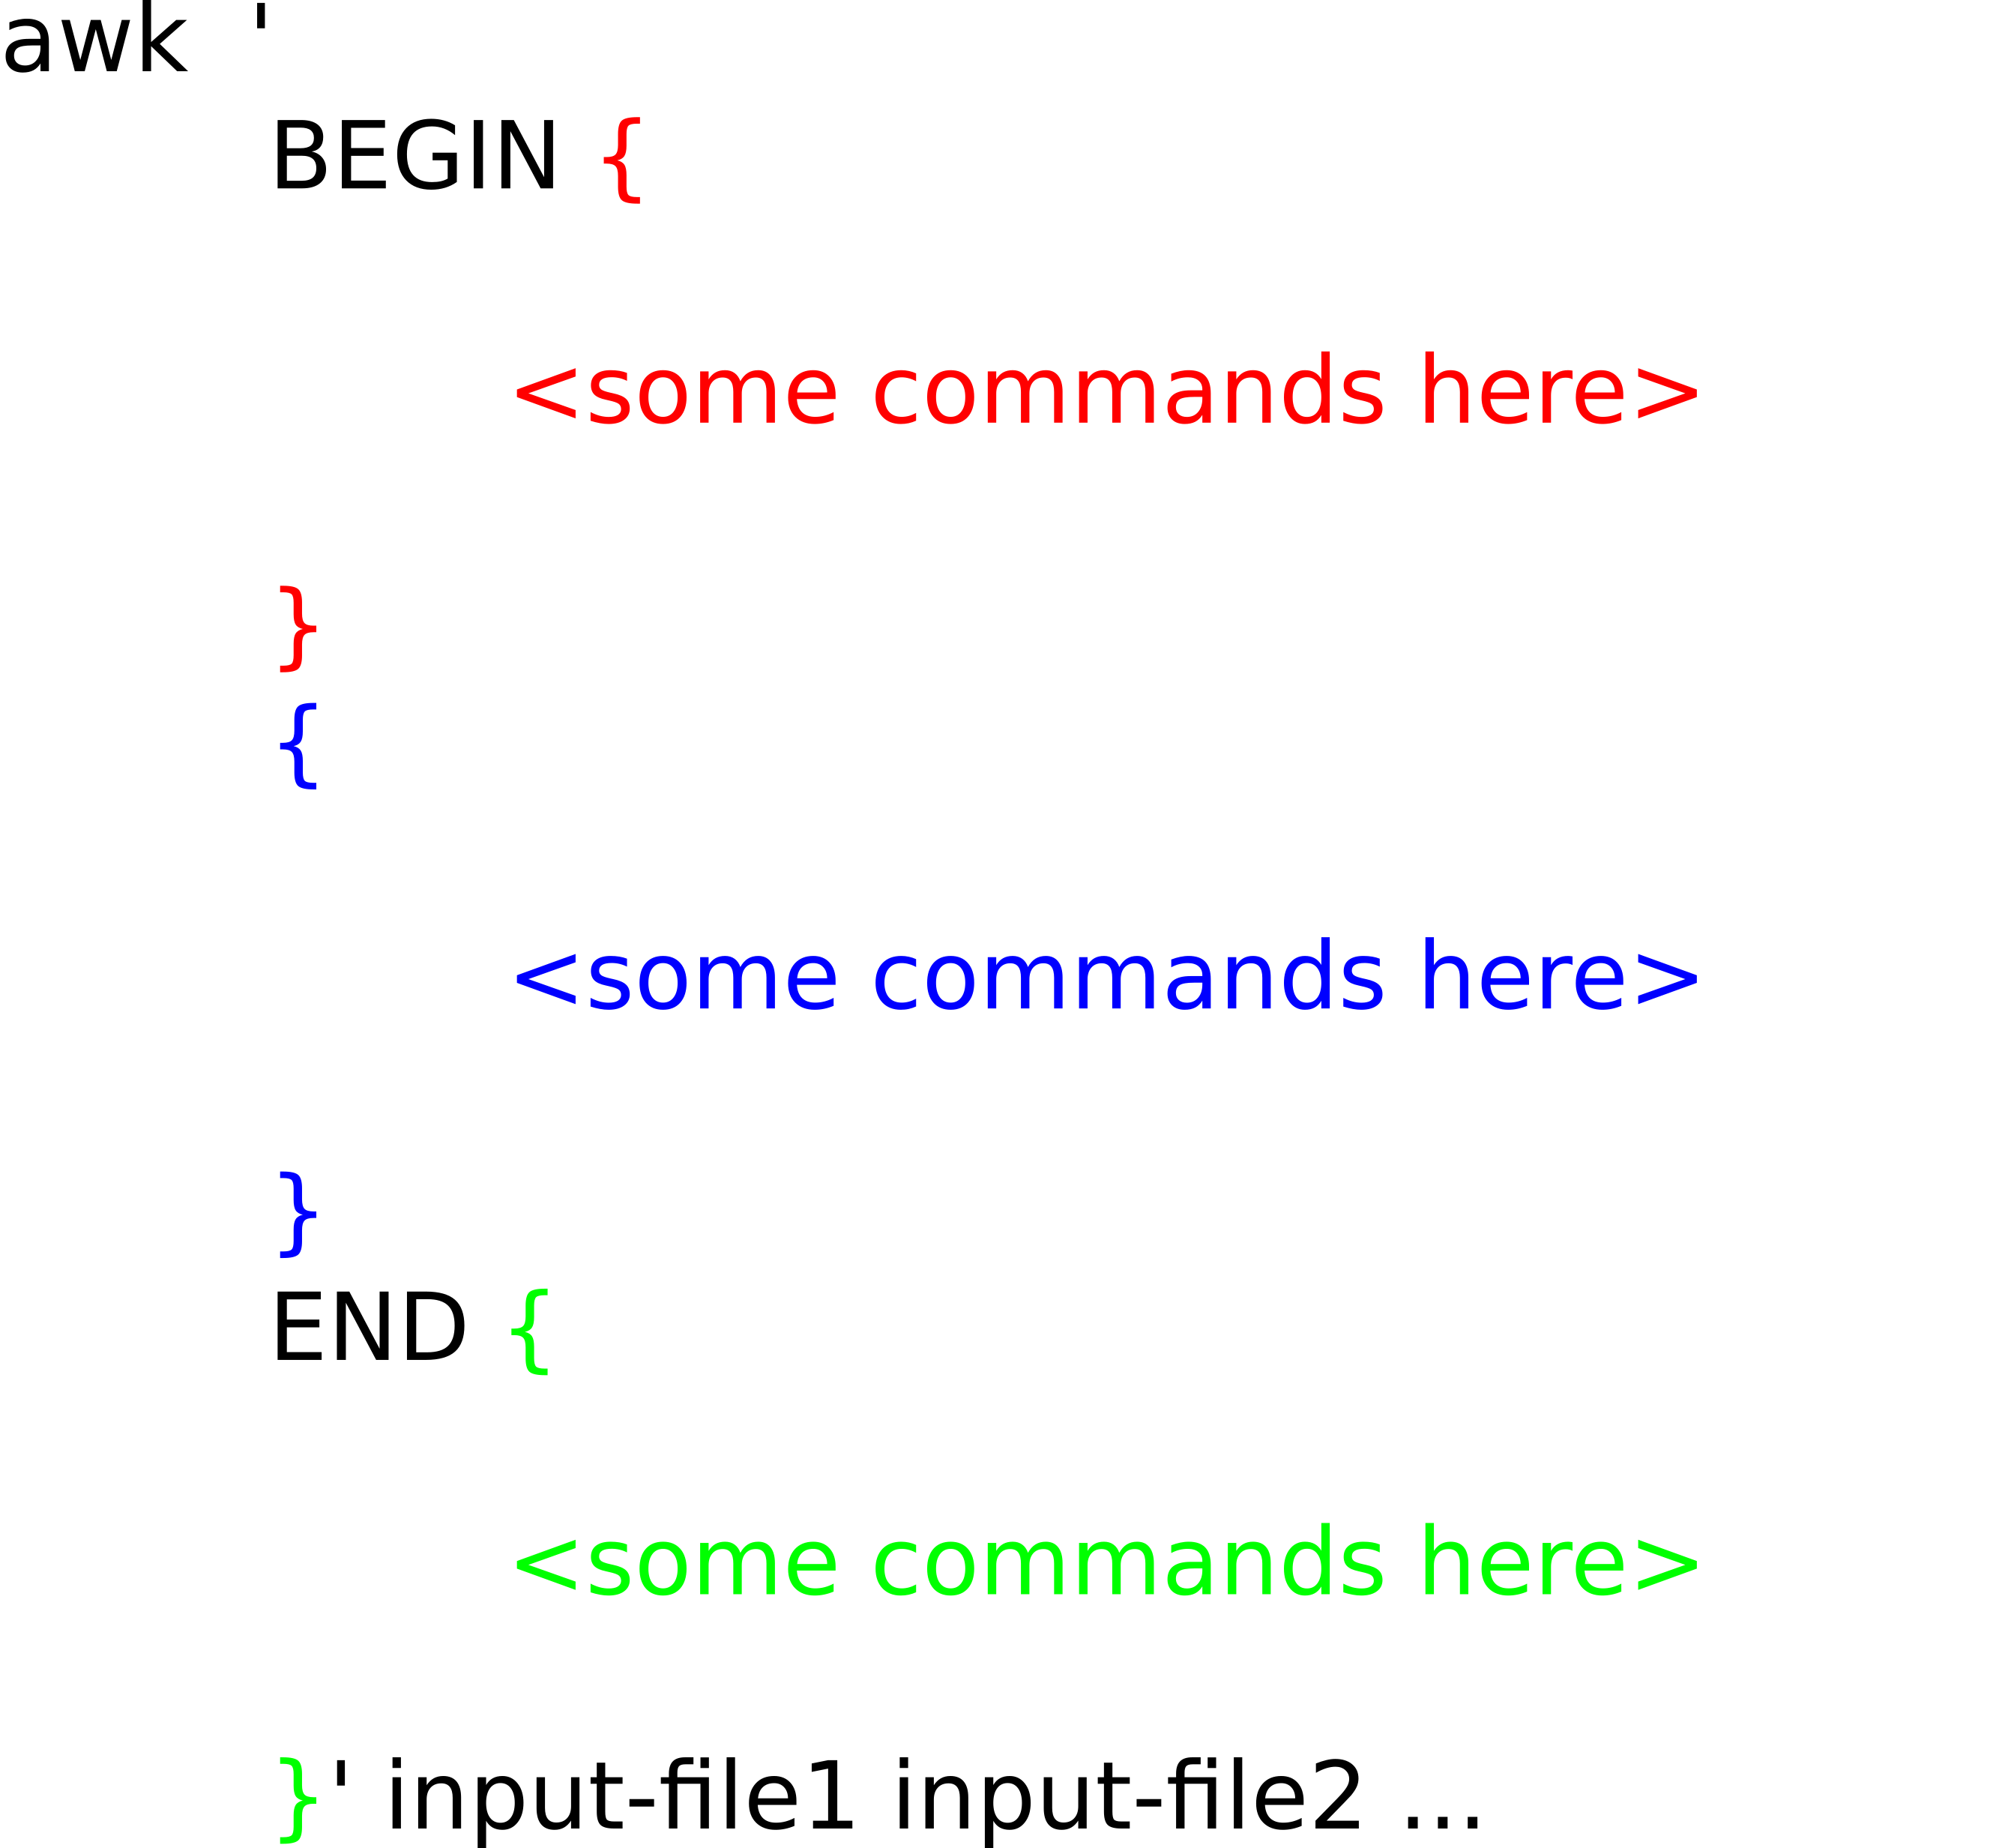
\includegraphics[scale=0.32,keepaspectratio]{awkMultipleInput.png}
    \end{figure}
    \iffalse {
    \begin{enumerate}
        \item BEGIN block (if present) gets executed only once before the first record is read.
        \item AWK reads file1 completely and looks for patterns. If found, the commands are executed for file1. The variables declared within the command block can be accessed by each file. In other words, they are not automatically reset when AWK finishes the current file and is about to read the next file.
        \item AWK reads file2 completely and so on.
        \item END block gets executed only once after all the files have been read.
    \end{enumerate}
    }
    \fi
\end{frame}
\begin{frame}
    \frametitle{Multiple input files - command line examples}
    \begin{itemize}
        \item FNR - total number of records processed until this point in the current file. If there are multiple input files this value gets reset to 0 at the beginning of a new file. Common first column example.
        \item FILENAME - contains the name of the file currently being read. If there are multiple input files this value gets updated at the beginning of a new file. Examples with grep for simple cases and AWK for more complicated cases.
        \item Assigning multiple values to the same variable for multiple files.
    \end{itemize}
\end{frame}
\begin{frame}
    \frametitle{AWK script files}
    \begin{itemize}
        \item Create a separate file with lots of commands.
        \item Can be run using two methods. 1) awk -f source-file input-file1 input-file2 ... 2) Make the source file executable using chmod.
        \item Comments - lines starting with the `\#' symbol.
    \end{itemize}
\end{frame}
\begin{frame}
    \frametitle{AWK script files}
    More predefined variables:
    \begin{itemize}
        \item ARGC - total number of arguments in the command line (including the key word awk and any variables that you might have declared).
        \item ARGV - array containing all the command line arguments.
        \item ARGIND - index of command line argument.
    \end{itemize}
\end{frame}
\begin{frame}
    \frametitle{AWK script files for processing data}
    \begin{itemize}
        \item Few examples combining shell commands with AWK.
    \end{itemize}
\end{frame}
\begin{frame}
    \frametitle{When to use AWK}
    ``Now that you’ve seen some of what awk can do, you might wonder how awk could be useful for you. By using utility programs, advanced patterns, field separators, arithmetic statements, and other selection criteria, you can produce much more complex output. The awk language is very useful for producing reports from large amounts of raw data, such as summarizing information from the output of other utility programs like ls."\\
    \vspace{2cm}
    \begin{center}
        \tiny{Source: https://www.gnu.org/software/gawk/manual/gawk.html}
    \end{center}

\end{frame}
\end{document}
